\begin{frame}{Adaptivity on Sparse Grids}{Types of Adaptivity}

    \begin{itemize}[<+->]
        \item A regular sparse grid is constructed in a way that takes a cut in diagonal hyperplane.
        \item All the dimensions and regions are assumed to be equally important.
        \item Adaptivity provides a smaller error with the same number of grid points.
        \item Adaptation criteria play an important role.
    \end{itemize}

    \begin{columns}
        \pause
        \begin{column}{0.5\textwidth}
            \begin{center}
                \textbf{Dimensional Adaptivity}
            \end{center}
            \begin{itemize}[<+->]
                \item Can be used when \(f\) has a different characteristic in different dimensions.
            \end{itemize}
        \end{column}
        \pause
        \begin{column}{0.5\textwidth}
            \begin{center}
                \textbf{Spatial Adaptivity}
            \end{center}
            \begin{itemize}[<+->]
                \item Can be used when \(f\) has a different characteristic in specific regions
            \end{itemize}
        \end{column}
    \end{columns}

\end{frame}

\begin{frame}{Adaptivity on Sparse Grids}{Spatial Adaptivity}
    \begin{itemize}[<+->]
        \item[]    Consider a function \(f\) such that it is mostly flat expect a region in the domain.
        \item[] Let say the region is near \( (0.4,0.6) \).
        \item[] A regular or dimensionally adaptive sparse grid would require many points to capture the local behaviour of \(f\) near \( (0.4,0.6) \).
        \item[] The point where \(f\) is mostly flat are wasted.
        \item[] Spatial adaptivity allows to use more grid points locally.
    \end{itemize}

\end{frame}

\begin{frame}{Adaptivity on Sparse Grids}{Adaptivity Criterion}

    \begin{columns}
        \begin{column}{0.5\textwidth}
            \begin{figure}
                \centering
                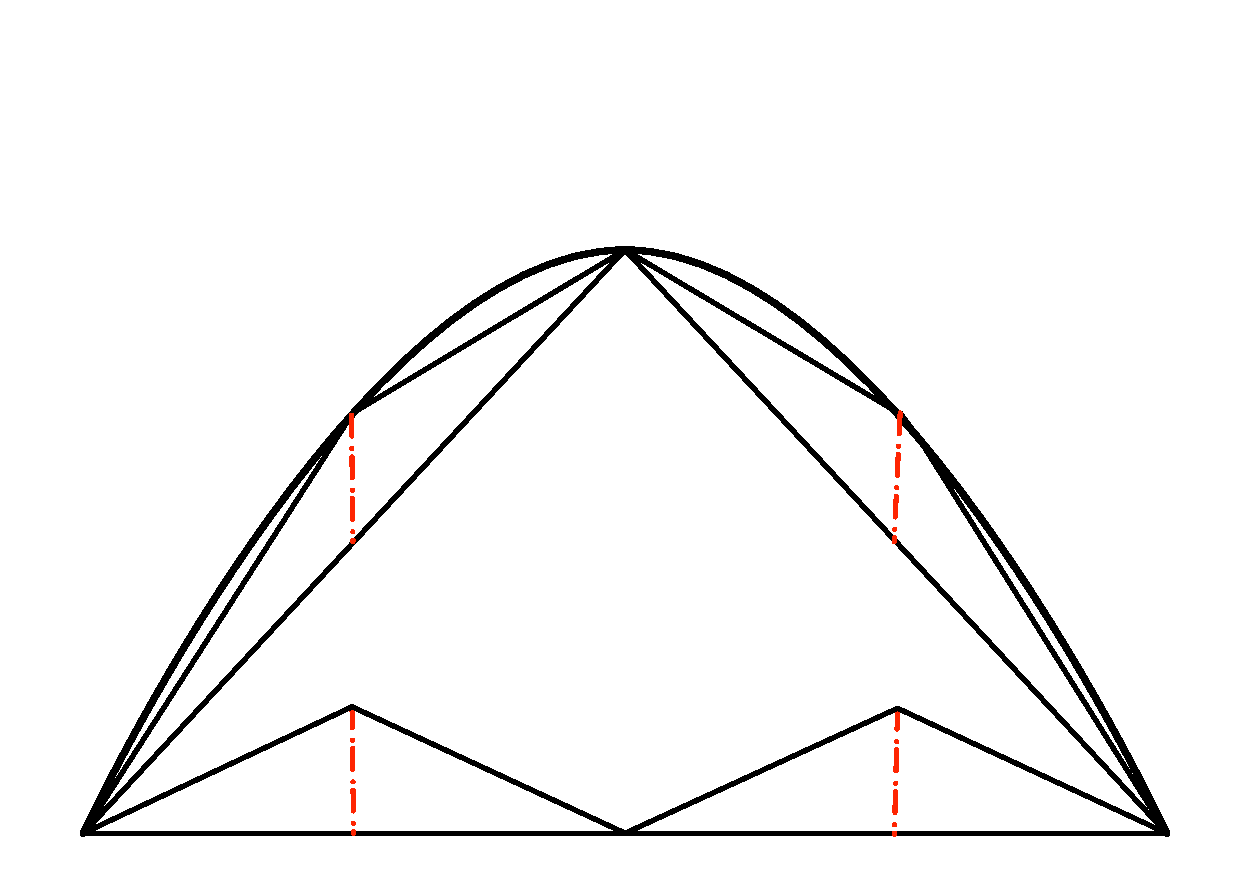
\includegraphics[width=\textwidth,height=0.5\textheight,keepaspectratio]{figures/surplus_interpolation.pdf}
                \caption{Interpolation of a parabola using 2 level hierarchical basis and surpluses, surpluses are shown in red lines.}
            \end{figure}
        \end{column}
        \begin{column}{0.5\textwidth}
            \begin{itemize}[<+->]
                \item One of the popular criterion is so called \emph{surplus-based criterion}.
                \item  It uses the absolute values of of hierarchical surpluses \(\vb{\alpha}\), to estimate second derivative of the function \(f\). In general, a larger absolute surplus means a larger second derivative.
                \item  More grid points are inserted to vicinity of larger surplus values.
            \end{itemize}
        \end{column}
    \end{columns}

\end{frame}

\begin{frame}{Adaptivity on Sparse Grids}{Spatial Adaptivity Requirements}
    The requirements for spatial adaptivity can be listed as follows:
    \begin{itemize}[<+->]
        \item An initial coarse grid.
        \item Iteratively choose region of interests.
        \item Add new points to region of interests.
        \item The grid should contain all the hierarchical ancestors of all grid points.
        \item Due to the consistency constraint, the number of points added can be larger than \(2 \cdot d\).
    \end{itemize}
\end{frame}

\begin{frame}{Adaptivity on Sparse Grids}{Spatial Adaptivity in Action}
    \begin{columns}
        \begin{column}{0.5\textwidth}
            \begin{figure}
                \centering
                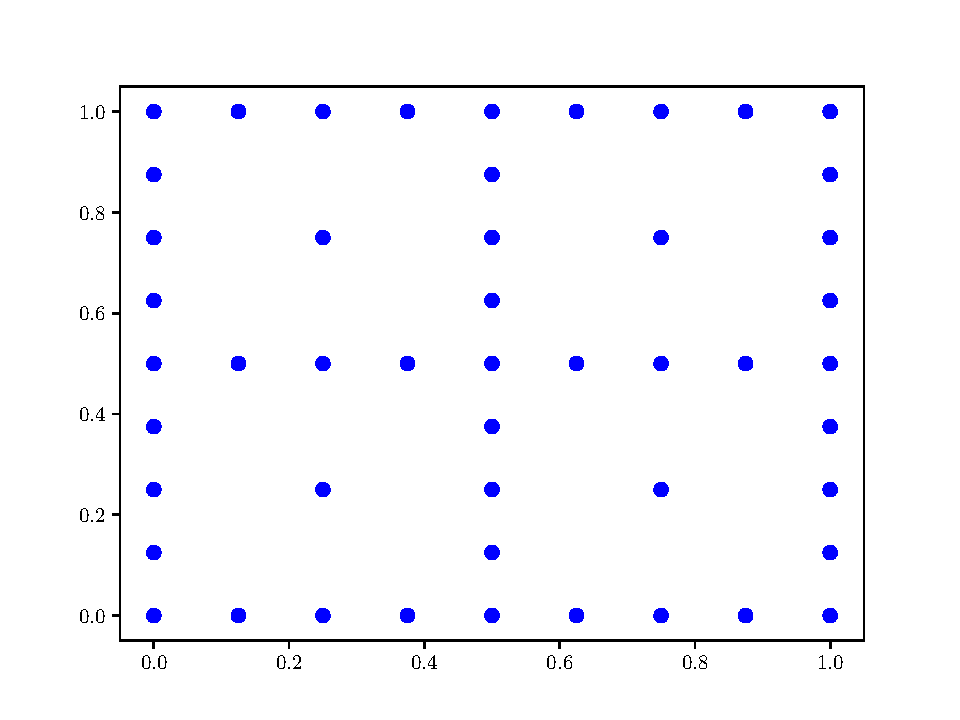
\includegraphics[width=\textwidth]{figures/before_refinement.pdf}
                \caption{Level 3 Regular grid \textcolor{red}{before} adaptation.}
            \end{figure}
        \end{column}
        \begin{column}{0.5\textwidth}
            \begin{figure}
                \centering
                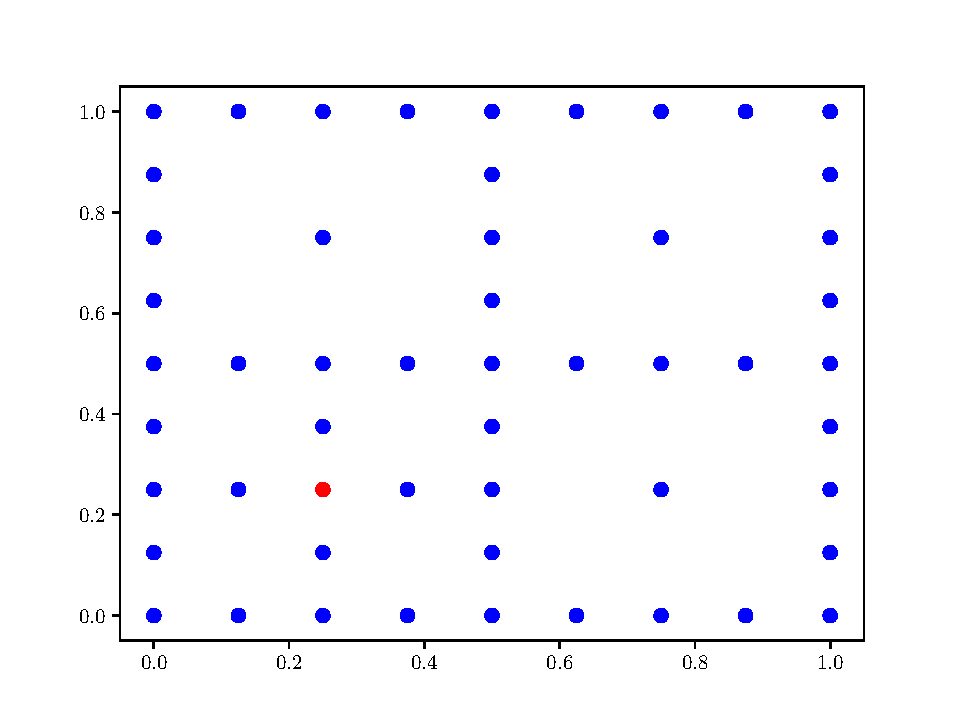
\includegraphics[width=\textwidth]{figures/refinement_0.pdf}
                \caption{Level 3 Regular grid \textcolor{red}{after} adaptation.}
            \end{figure}
        \end{column}
    \end{columns}
\end{frame}